% Options for packages loaded elsewhere
\PassOptionsToPackage{unicode}{hyperref}
\PassOptionsToPackage{hyphens}{url}
%
\documentclass[
]{article}
\usepackage{lmodern}
\usepackage{amssymb,amsmath}
\usepackage{ifxetex,ifluatex}
\ifnum 0\ifxetex 1\fi\ifluatex 1\fi=0 % if pdftex
  \usepackage[T1]{fontenc}
  \usepackage[utf8]{inputenc}
  \usepackage{textcomp} % provide euro and other symbols
\else % if luatex or xetex
  \usepackage{unicode-math}
  \defaultfontfeatures{Scale=MatchLowercase}
  \defaultfontfeatures[\rmfamily]{Ligatures=TeX,Scale=1}
\fi
% Use upquote if available, for straight quotes in verbatim environments
\IfFileExists{upquote.sty}{\usepackage{upquote}}{}
\IfFileExists{microtype.sty}{% use microtype if available
  \usepackage[]{microtype}
  \UseMicrotypeSet[protrusion]{basicmath} % disable protrusion for tt fonts
}{}
\makeatletter
\@ifundefined{KOMAClassName}{% if non-KOMA class
  \IfFileExists{parskip.sty}{%
    \usepackage{parskip}
  }{% else
    \setlength{\parindent}{0pt}
    \setlength{\parskip}{6pt plus 2pt minus 1pt}}
}{% if KOMA class
  \KOMAoptions{parskip=half}}
\makeatother
\usepackage{xcolor}
\IfFileExists{xurl.sty}{\usepackage{xurl}}{} % add URL line breaks if available
\IfFileExists{bookmark.sty}{\usepackage{bookmark}}{\usepackage{hyperref}}
\hypersetup{
  pdftitle={Homework 02},
  pdfauthor={Ming Lin},
  hidelinks,
  pdfcreator={LaTeX via pandoc}}
\urlstyle{same} % disable monospaced font for URLs
\usepackage[margin=1in]{geometry}
\usepackage{graphicx}
\makeatletter
\def\maxwidth{\ifdim\Gin@nat@width>\linewidth\linewidth\else\Gin@nat@width\fi}
\def\maxheight{\ifdim\Gin@nat@height>\textheight\textheight\else\Gin@nat@height\fi}
\makeatother
% Scale images if necessary, so that they will not overflow the page
% margins by default, and it is still possible to overwrite the defaults
% using explicit options in \includegraphics[width, height, ...]{}
\setkeys{Gin}{width=\maxwidth,height=\maxheight,keepaspectratio}
% Set default figure placement to htbp
\makeatletter
\def\fps@figure{htbp}
\makeatother
\setlength{\emergencystretch}{3em} % prevent overfull lines
\providecommand{\tightlist}{%
  \setlength{\itemsep}{0pt}\setlength{\parskip}{0pt}}
\setcounter{secnumdepth}{-\maxdimen} % remove section numbering
\ifluatex
  \usepackage{selnolig}  % disable illegal ligatures
\fi

\title{Homework 02}
\author{Ming Lin}
\date{}

\begin{document}
\maketitle

I pledge my honor that I have abided by the Stevens Honor System

Problem 1(i)

For, n = 20, P(N \textless= 8.5) = 0.5955987\\
For, n = 30, P(N \textless= 8.5) = 0.0940112\\
For, n = 50, P(N \textless= 8.5) =
\ensuremath{2.3052286\times 10^{-4}}\\
For, n = 75, P(N \textless= 8.5) = \ensuremath{1.826106\times 10^{-8}}\\
For, n = 100, P(N \textless= 8.5) =
\ensuremath{5.4311266\times 10^{-13}}

Problem 1(ii)

For, n = 20, P(N \textless= 8.5) = 0.6331\\
For, n = 30, P(N \textless= 8.5) = 0.0606\\
For, n = 50, P(N \textless= 8.5) = 0.00058\\
For, n = 75, P(N \textless= 8.5) = 1.475e\^{}-7 ~\\
For, n = 100, P(N \textless= 8.5) = 8.91e\^{}-11

Problem 1(iii)

\begin{flushleft}\includegraphics[width=0.5\linewidth,height=0.5\textheight]{hw02_files/figure-latex/unnamed-chunk-3-1} \end{flushleft}

Problem 1(iv)\\
As the errors downtrend to nearly but not 0, the N increases.

Problem 2

\begin{verbatim}
## [1] "N = 20"
\end{verbatim}

\includegraphics[width=0.3\linewidth]{hw02_files/figure-latex/unnamed-chunk-5-1}
\includegraphics[width=0.3\linewidth]{hw02_files/figure-latex/unnamed-chunk-5-2}
\includegraphics[width=0.3\linewidth]{hw02_files/figure-latex/unnamed-chunk-5-3}

\begin{verbatim}
## [1] "N = 30"
\end{verbatim}

\includegraphics[width=0.3\linewidth]{hw02_files/figure-latex/unnamed-chunk-5-4}
\includegraphics[width=0.3\linewidth]{hw02_files/figure-latex/unnamed-chunk-5-5}
\includegraphics[width=0.3\linewidth]{hw02_files/figure-latex/unnamed-chunk-5-6}

\begin{verbatim}
## [1] "N = 50"
\end{verbatim}

\includegraphics[width=0.3\linewidth]{hw02_files/figure-latex/unnamed-chunk-5-7}
\includegraphics[width=0.3\linewidth]{hw02_files/figure-latex/unnamed-chunk-5-8}
\includegraphics[width=0.3\linewidth]{hw02_files/figure-latex/unnamed-chunk-5-9}

\begin{verbatim}
## [1] "N = 75"
\end{verbatim}

\includegraphics[width=0.3\linewidth]{hw02_files/figure-latex/unnamed-chunk-5-10}
\includegraphics[width=0.3\linewidth]{hw02_files/figure-latex/unnamed-chunk-5-11}
\includegraphics[width=0.3\linewidth]{hw02_files/figure-latex/unnamed-chunk-5-12}

Problem 2(v)

After observing the plots, I notice that the values seem to peak in the
middle and through sample size n that throughout each graph their slope
and pattern are similar

Problem 2(vi)

After observing the scatter plots, I noticed that the values are
uniformly randomly distributed in the middle of the scatter plot. Also,
the scatter plot shows minimal correlation and increasing density in the
middle.

Problem 3

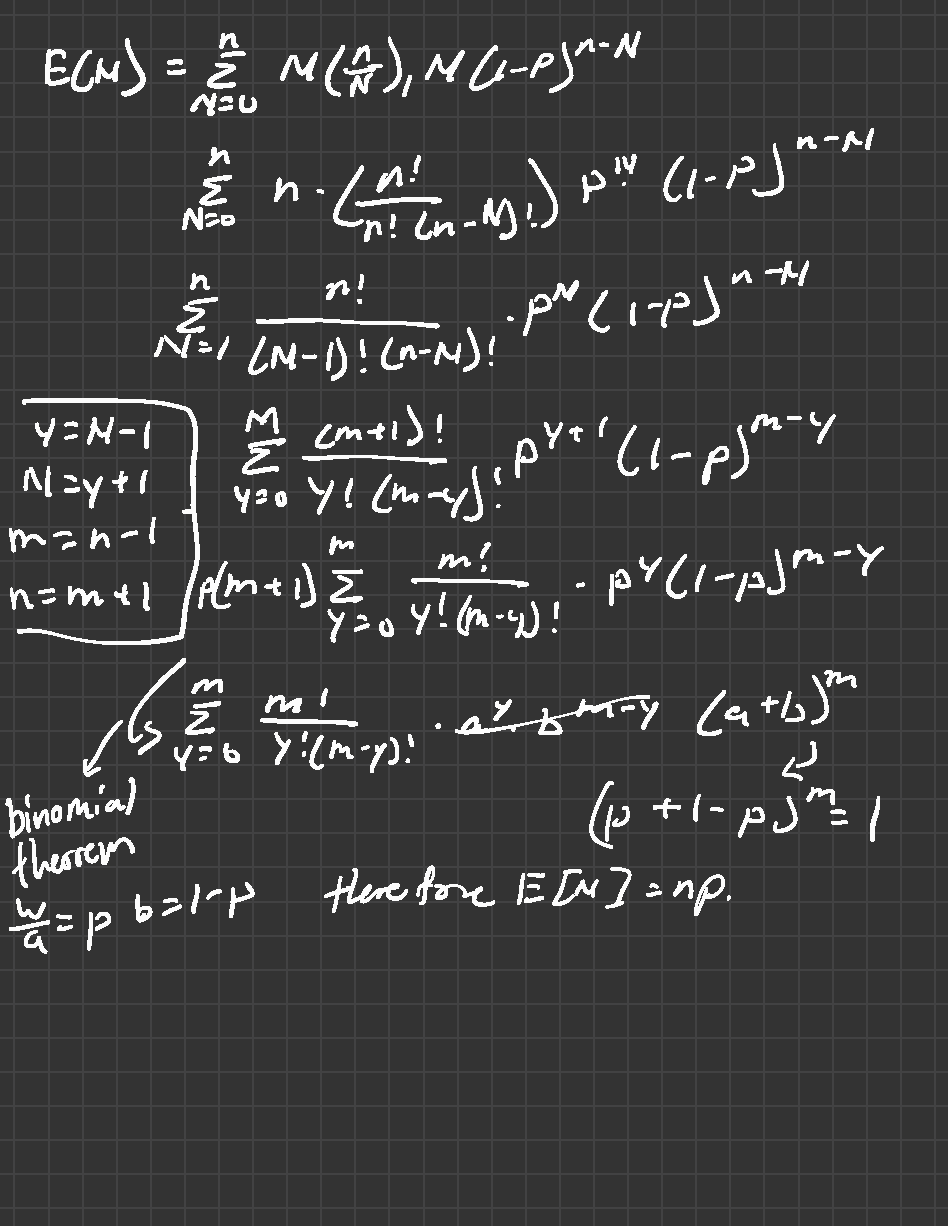
\includegraphics{/Users/minglin/Stevens-IT/MA331/hw02/prob3.pdf}

Problem 4

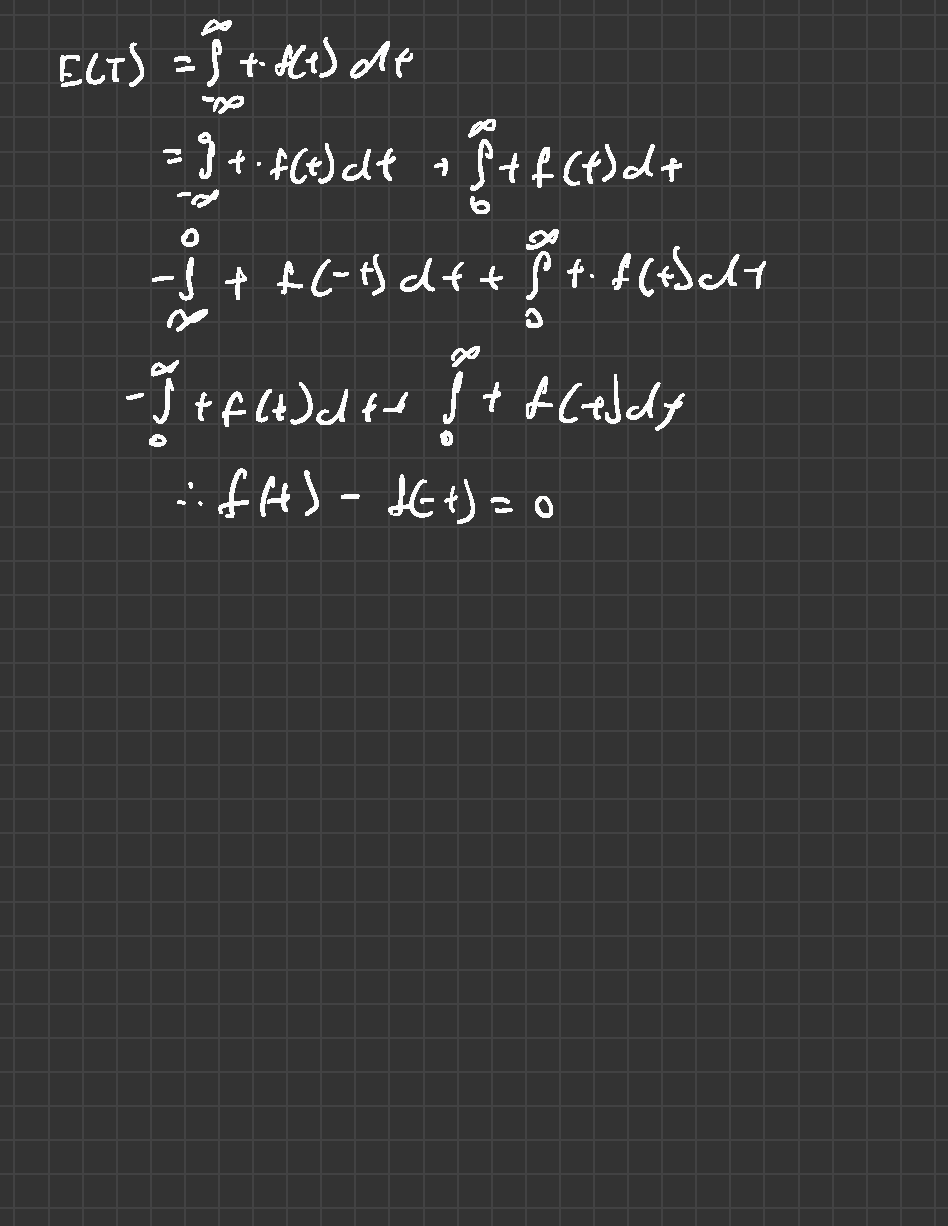
\includegraphics{/Users/minglin/Stevens-IT/MA331/hw02/prob4.pdf}

\end{document}
